\Def Уравнение $f(x) = 0$ \textbf{разрешимо в радикалах} над $\Q$, если выполнено одно из следующих условий:

\begin{enumerate}
\item $\exists$ $\alpha$ - корень многочлена $f(x)$: $\alpha \in K = K_0 \supset K_1 \supset \dots \supset K_n = \Q$; $K_i = K_{i+1}(a_i), a_i^{m_i} \in K_{i+1}$ 
\item $\forall$ $\alpha$ - корень многочлена $f(x)$: $\alpha \in K = K_0 \supset K_1 \supset \dots \supset K_n = \Q$; $K_i = K_{i+1}(a_i), a_i^{m_i} \in K_{i+1}$

\end{enumerate}

\Note Вместо $\Q$ может быть любое другое поле.

\Note Идейно мы хотим сказать, что разрешимо в радикалах - значит, можно получить ответ при помощи операция $+, -, \cdot, \backslash$ и $\sqrt[n]{}$

\Note Из 1 следует 2 (и наоборот, очев), но док-во технически сложное и не приводится. 

\Note Проблемы с определением 1: хотим, чтобы $K$ было нормальным над $\Q$; так же хочется, чтобы K было похоже на поле разложения многочлена.

Отсюда 3 определение: $K_i$ - поле разложения $x^{m_i} - a_i$ над $K_{i+1}$.

Не решает первую проблему, т.к. \Example 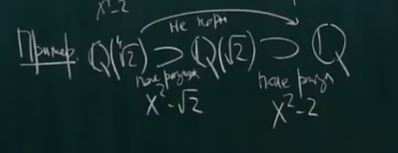
\includegraphics[]{images/5_19.JPG}

\textbf{Идея:} также брать $x^{m_i} - \overline{a_i}$ для всех сопряжённых к $a_i$.

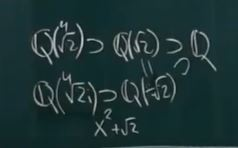
\includegraphics[]{images/5_19_2.JPG}

\Th $f(x) = 0$ разрешимо в радикалах $\Leftrightarrow$ Существует башня расширений $L = L_0 \supset L_1 \supset \dots \supset L_n = \Q$ такая, что для каждого $i \in \{0, 1, \dots, n-1 \}$ поле $L_i$ — это поле разложения многочлена $x^{m_{i+1}} - a_{i+1} \in L_{i+1}[x]$ (одно из определений разрешимости в радикалах)

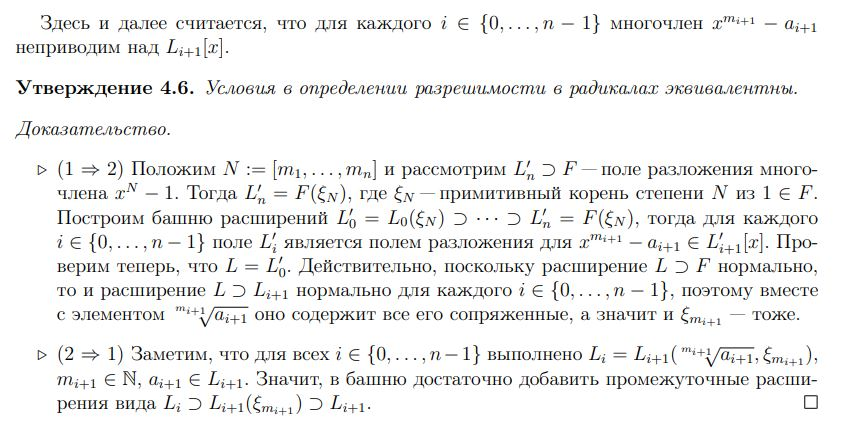
\includegraphics[]{images/5_19_3.JPG}